\documentclass{article}
\usepackage[utf8]{inputenc}
\usepackage{slashed}
\usepackage{graphicx}
\usepackage{amssymb}
\usepackage{amssymb,latexsym}
\usepackage{amsmath,amsbsy,bbm}
\usepackage{multirow}

\usepackage[vcentermath]{youngtab}

\newcommand{\eftnopi}{\mbox{$\slashed{\pi}$EFT }} 



\title{JLM-Machester}
\author{J K \& L C}
\date{October 2018}

\begin{document}

\maketitle

\section{Problem(s)}
What follows is a rigorous definition of problems, this work aims to formulate an
answer for:
\begin{itemize}
    \item Can a two-body, momentum-independent contact interaction generate renormalization-group
    invariant structure close to ``some'' threshold of an amplitude which demands the contribution
    from at least one asymmetric spacial state?
\end{itemize}

\begin{description}
\item[16.10.2018] $$\lim\limits_{\Lambda\to\infty}B_c(2)=\infty$$ In words, the critical two-neutron binding
energy, which is attained by an enhancement of the two LO contact interactions which is surpassed by an
eigenvalue with $J^\pi=\frac{1}{2}^-$ in the three-neutron space, diverges.

The calculations I did were different when enhancing a P-wave interaction -- Tensor and/or spin-orbit times 
a delta function. The LO contacts are kept constant and the critical values pertain to the
emergent ${}^3P_J$ bound states.

\item[17.10.2018] Negative-parity two-body matrix elements vanish for zero-range interactions
because Legendre polynomials of odd order are zero for $\cos\theta=0$. Matrix elements involving more
than two neutrons do not vanish in that limit which is shown in Fig.~(2) of~\cite{Kirscher:2017xpj}
(the rest of this reference is to be ignored). 

\item[18.10.2018] The results of a ${}^2n-n$ scattering calculation at $m_\pi=806~$MeV,
with $\Lambda\in\lbrace6,12,15\rbrace~\textrm{fm}^{-1}$, and  $C_S=C_T$ such that
$B({}^2n)\in\lbrace19,\mathcal{O}(5),\lesssim 1\rbrace~\textrm{MeV}$.
The phase shifts are calculated for center-of-mass energies between the neutron projectile
and the dineutron ${}^1S_0$ target that do not exceed the breakup energy by much (for the lighter bound
dineutrons). The channel quantum numbers are $J^\pi=\frac{1}{2}^-$.

The behavior does not indicate the presence of a pole of the S matrix the steeper rise for shallower
dineutron, i.e., a two-body interaction closer to unitarity, is a consequence of the nearby breakup
threshold, i.e., a branch cut.

Binding energy calculations with appropriate boundary conditions do not yield anything insightful
either.

At this point, I would now continue with arguments as sketched in the infamous manuscript, and claim
that the apparently non-vanishing P-wave attraction between the neutron and the dimer is statistically
enhanced for the neutron trimer effective interaction.

{\bf Any thoughts?} I am forced to work on Compton scattering, now. Let us talk on your Tuesday, which
is my Monday, which is the day until which we could resovle the problem :)

\end{description}


\section{Introduction}
As of now, the pionless EFT constitutes the minimal theory which can predict the behavior of
two nucleons at low energy with arbitrary accuracy. A similarly renormalization-scheme independent
theory has not yet been formulated for nuclear properties which involve more than four interacting
nucleons. Even the consistency of the pionless theory in the four-nucleon system is supported by
numerical results, only.

Here, we conjecture a minimal theory based on the pionless EFT which is useful in the sense that
it predicts the mass gap in the five-nucleon system and correlates the bound cluster structure of
$^{16}$O to $A\leq4$ observables.

Since the first attempts to extend the \eftnopi (pionless effective field theory) to the four-body system \cite{Barnea:2013uqa}, physicist question the possibility to describe system with P-wave ($L=$1) components in the wave function using just a S-wave contact approach.
In nuclear physics, those systems are represented by $A\ge$5, however, the unbound nature of the five-nucleon system and the halo nature of the six-body nucleon makes this problem difficult to be investigated using a realistic \eftnopi.
Nevertheless, attempts to study the problem have been made in $^6$Li \cite{Barrett:2012dr}, and in $^{16}$O \cite{Contessi:2017rww}.
In the first case the results are encouraging, however, the small cut-offs considered make the results not completely conclusive.
In the second case no sign of bound oxygen is found and the system result not stable against four-$\alpha$ breaking, also in this case the study is not conclusive, since the binding energy of $^{16}$O is only 10\% larger than the four-$\alpha$ threshold, well inside the truncation error of the theory at LO.

In this work we study the behaviour of LO S-wave \eftnopi applied to P-wave systems.
To avoid the difficulties of working in unbound or halo nuclear systems a toy \eftnopi is created to demonstrate the \textit{possibility} to bind P-wave systems with S-wave contact interaction.
If this is not possible the only chance to describe P-wave systems in \eftnopi might be to introduce explicit P-wave poles in the LO T-matrix \cite{BERTULANI200237}.

\section{Pionless interaction}
The two-body interaction we are using is:

\begin{equation}
    V(r_{ij})=C_{1^S_0}^\Lambda P_{1^S_0} e^{-\frac{r_{ij}^2\Lambda}{4}} + 
              C_{3^S_1}^\Lambda P_{3^S_1} e^{-\frac{r_{ij}^2\Lambda}{4}}
\end{equation}

The three-body one is:
\begin{equation}
    V(r_i,r_j,r_k)=D_0^\Lambda \sum_{cyc} \left[ e^{-\frac{\left(r_{ij}^2+r_{ik}^2\right)\Lambda}{4}} \right] 
\end{equation}

where $P$ represent the spin/isospin projection in one of the possible channels allowed by the antisymmetrization of four-spinor fermions. 


\section{List of possible calculations}

Performing the calculation for physical pion mass might be the best choice to convince peoples that what is done is applicable also in standard nuclear physics.
Therefore the nucleon mass can be set to $938.95$ MeV and $\frac{\hbar^2}{m}=41.4709931$.
The parameters are:

\begin{center}
\begin{tabular}{  c c c c }
 $\lambda$   &  $C_{^1S_0}$ &  $C_{^3S_1}$ &    D \\
4            & -434.958473  &	-505.1643  &	677.7989\\
                       6            & -986.251897  &	-1090.584  &	2652.651\\
                       8            & -1760.16173  &	-1898.622  &	7816.228\\
\end{tabular}
\end{center}

We are not probably interested in spin dependence so we can take only the central part of the interaction:

\begin{center}
\begin{tabular}{ c c c }
 $\lambda$   &   $C$      &    D \\
4            & -487.6128  &	677.7989\\
6            & -1064.5010 & 2652.651\\
8            & -1864.0069 & 7816.228\\
\end{tabular}
\end{center}

to check the dependence from the lecs we might try a couple of different configurations like double and half:

\begin{center}
\begin{tabular}{ c c c c }
& $\lambda$   &   $C$      &    D \\
\multirow{3}{*}{double}& 4            & -487.6128  &	677.7989\\
& 6            & -1064.5010 & 2652.651\\
& 8            & -1864.0069 & 7816.228\\
\end{tabular}
\end{center}

Interesting systems are:

\begin{center}
\begin{tabular}{ c c c }
$^3n$=\yng(2,1) & $^5He$=\yng(4,1)\\
$^4n$=\yng(2,2) & $^6He$=\yng(4,2)\\
\end{tabular}
\end{center}

whose require also the calculation of $d$=\yng(2) and $^4He$=\yng(4) to check the treshold energies.
\section{n-n-n system}
The first step taken in order to apply \eftnopi to P-wave systems is to examine $nn$ and $nnn$ systems, where only spin singlet two-body contact interaction is finite and $C_{1^S_0}$ is the only degree of freedom of the system.
If fitted on experimental data \cite{} for a cut-off $\Lambda=6$ fm$^{-1}$, $C_{1^S_0}^6=$-982.06 MeV (As comparison $C_{3^S_1}^6=$-1090.584 MeV).


\begin{figure}[h] 
\centering 
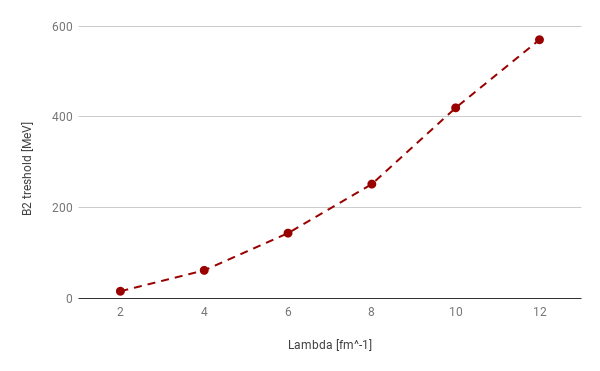
\includegraphics[width=0.8\textwidth]{./2b_3b_treshold} 
\caption{Two-body binding energy at which the three body system becomes bound in function of the cut off.} 
\end{figure} 

\begin{figure}[h] 
\centering 
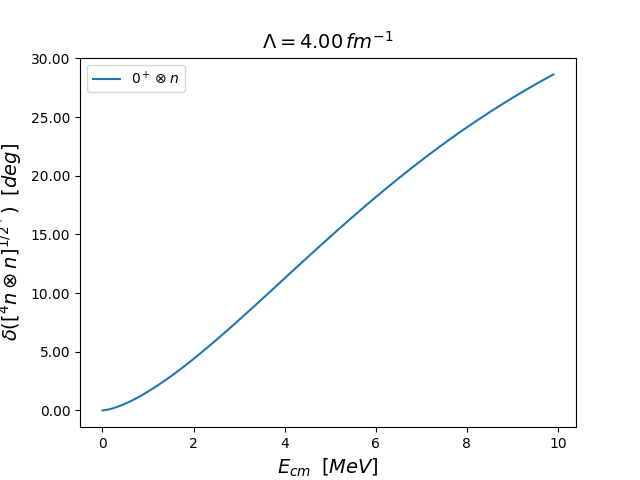
\includegraphics[width=0.8\textwidth]{./Figure_4.png} 
\caption{Phase shift for neutron$-\alpha$ scattering at physical $m_\pi$.} 
\end{figure}

The data sown that increasing the cut-off the binding energy at which $nnn$ increases as a positive power of the cut-off meaning that this three body state is an artifact of the renormalization scheme and it is not possible to represent such state with a S-wave contact theory. 
As a result, the only way to describe this system might be to introduce a p-wave pole directly in the two body scattering matrix or to include an attractive three-body p-wave interaction.


\section{n-$\alpha$ system}

\section{Dimer-Dimer EFT}

Petrov showed in \cite{petrov_dimerov} that dimeron dimeron is not bound having a scattering length that is 0.6 with respect to the nn system with zero range s-wave interaction.
In another paper \cite{petrov_dimerov_nm} he shows something about dimerons with different masses but I need to read the paper (but I think the answere is yes). 

What I ask myself is: if I have dimeron dimeron interaction that binds the d-d system, where is the difference with respect to the contact s-wave?

I write the dibarion formalism assuming a pole in the dd system and I expand the theory assuming the fourn-neutron system to be $\alpha$:

\begin{align*}
    \mathcal{L}= & \, n^{\dag}_\uparrow\left(i\partial_0+\frac{\nabla^2}{2m}\right)n_\uparrow+n^{\dag}_\downarrow\left(i\partial_0+\frac{\nabla^2}{2m}\right)n_\downarrow+\\
    &\, d^{\dag}\Delta_dd+g^2_d\left( d^{\dag}nn+n^\dag n^\dag d \right)+\\
    &\, \alpha^\dag\Delta_\alpha\alpha+g^2_\alpha\left(\alpha^\dag dd+d^\dag d^\dag \alpha\right)\\
\end{align*}

if I perform a gaussian integration i get:

\begin{align*}
    \mathcal{L}= & \, n^{\dag}_\uparrow\left(i\partial_0+\frac{\nabla^2}{2m}\right)n_\uparrow+n^{\dag}_\downarrow\left(i\partial_0+\frac{\nabla^2}{2m}\right)n_\downarrow+\\
    &\, d^{\dag}\Delta_dd+g^2_d\left( d^{\dag}nn+n^\dag n^\dag d \right)+\frac{g^2_\alpha}{\Delta_\alpha} d^{\dag} d^{\dag}dd\\
\end{align*}

if I try to perform a new gaussian integration I get stuck with $\frac{g^2_\alpha}{\Delta_\alpha} d^{\dag} d^{\dag}dd$ which is not quadratic nor linear, and I guess that would give some non s-wave therms in the $n^\dag n^\dag n n$ therms.

This makes the issue explicit which we sketched on the white board recently, namely that beyond
three particles, the iterated out-integration is not a straight-forward Gaussian. Formally, could we
make use of the formula
$$\int_0^\infty~dx~x^n~e^{-a\cdot x^b}=b^{-1}a^{-\frac{n+1}{b}}~\Gamma\left(\frac{n+1}{b}\right)\;\;?$$



\section{Larger systems}


\section{Conclusions}

\newpage
\bibliographystyle{unsrt}
\bibliography{Thebibliography.bib}
\end{document}
